% Template LaTeX file for DAFx-20 papers
%
% To generate the correct references using TeX, run
%     latex, bibtex, latex, latex
% modified...
% - from DAFx-00 to DAFx-02 by Florian Keiler, 2002-07-08
% - from DAFx-03 to DAFx-04 by Gianpaolo Evangelista, 2004-02-07 
% - from DAFx-05 to DAFx-06 by Vincent Verfaille, 2006-02-05
% - from DAFx-06 to DAFx-07 by Vincent Verfaille, 2007-01-05
%                          and Sylvain Marchand, 2007-01-31
% - from DAFx-07 to DAFx-08 by Henri Penttinen, 2007-12-12
%                          and Jyri Pakarinen 2008-01-28
% - from DAFx-08 to DAFx-09 by Giorgio Prandi, Fabio Antonacci 2008-10-03
% - from DAFx-09 to DAFx-10 by Hannes Pomberger 2010-02-01
% - from DAFx-10 to DAFx-12 by Jez Wells 2011
% - from DAFx-12 to DAFx-14 by Sascha Disch 2013
% - from DAFx-15 to DAFx-16 by Pavel Rajmic 2015
% - from DAFx-16 to DAFx-17 by Brian Hamilton 2016
% - from DAFx-17 to DAFx-18 by Annibal Ferreira and Matthew Davies 2017
% - from DAFx-18 to DAFx-19 by Dave Moffat 2019
% - from DAFx-19 to DAFx-20 by Gianpaolo Evangelista 2019
%
% Template with hyper-references (links) active after conversion to pdf
% (with the distiller) or if compiled with pdflatex.
%
% 20060205: added package 'hypcap' to correct hyperlinks to figures and tables
%                      use of \papertitle and \paperauthorA, etc for same title in PDF and Metadata
% 20190205: Package 'hypcap' removed, and replaced with 'caption', to allow for the inclusion
%			of a CC UP licence.
%
% 1) Please compile using latex or pdflatex.
% 2) If using pdflatex, you need your figures in a file format other than eps! e.g. png or jpg is working
% 3) Please use "paperftitle" and "pdfauthor" definitions below

%------------------------------------------------------------------------------------------
%  !  !  !  !  !  !  !  !  !  !  !  ! user defined variables  !  !  !  !  !  !  !  !  !  !  !  !  !  !
% Please use the following commands to define title and author(s) of the paper.
% paperauthorA MUST be the the first author of the paper
% Please comment the unused definitions 
\def\papertitle{A Physical model of the Trombone using Dynamic Grids for Finite-Difference Schemes}
\def\paperauthorA{Silvin Willemsen}
\def\paperauthorB{Stefan Bilbao}
\def\paperauthorC{Michele Ducceschi}
\def\paperauthorD{Stefania Serafin}
%\def\paperauthorE{Author Five}
%\def\paperauthorF{Author Six}
%\def\paperauthorG{Author Seven}
%\def\paperauthorH{Author Eight}
%\def\paperauthorI{Author Nine}
%\def\paperauthorJ{Author Ten}

% Authors' affiliations have to be set below

%------------------------------------------------------------------------------------------
\documentclass[twoside,a4paper, dvipsnames]{article}
\usepackage{etoolbox}
\usepackage{dafx_20}
\usepackage{amsmath,amssymb,amsfonts,amsthm}
\usepackage{euscript}
%\usepackage[latin1]{inputenc}
\usepackage[T1]{fontenc}
\usepackage[utf8]{inputenc}
%\usepackage[T1]{fontenc}
%\usepackage{lmodern}
\usepackage{nimbusserif}
\usepackage{ifpdf}
\usepackage[english]{babel}
\usepackage{caption}
\usepackage{subfig} % or can use subcaption package
\usepackage{xcolor}
\usepackage{cases}
\usepackage{tikz}
\usetikzlibrary{decorations.markings}
\usepackage{algorithm2e, setspace}

\makeatletter
\renewcommand*\env@matrix[1][*\c@MaxMatrixCols c]{%
  \hskip -\arraycolsep
  \let\@ifnextchar\new@ifnextchar
  \array{#1}}
\makeatother

\def\SBcomment[#1]{\textcolor{Red}{}}
\def\SWcomment[#1]{\textcolor{Cyan}{}}
\def\MDcomment[#1]{\textcolor{PineGreen}{}}
\def\SScomment[#1]{\textcolor{Bittersweet}{}}
\DeclareMathAlphabet\mathbfcal{OMS}{cmsy}{b}{n}

\def\lg{{l}} % general l
\def\lp{{l_p}}
\def\lq{{l_q}}
\def\Nfrac{\mathcal{N}}
\def\flip{\leftarrow}
% \def\flip{\leftarrow}
% \def\U{\mathbfcal{U}}

\input glyphtounicode
\pdfgentounicode=1

\setcounter{page}{1}
\ninept

% build the list of authors and set the flag \multipleauth to handle the et al. in the copyright note (in DAFx_20.sty)
%==============================DO NOT MODIFY =======================================
\newcounter{numauth}\setcounter{numauth}{1}
\newcounter{listcnt}\setcounter{listcnt}{1}
\newcommand\authcnt[1]{\ifdefined#1 \stepcounter{numauth} \fi}

\newcommand\addauth[1]{
\ifdefined#1 
\stepcounter{listcnt}
\ifnum \value{listcnt}<\value{numauth}
\appto\authorslist{, #1}
\else
\appto\authorslist{~and~#1}
\fi
\fi}
%======DO NOT MODIFY UNLESS YOUR PAPER HAS MORE THAN 10 AUTHORS========================
%==we count the authors defined at the beginning of the file (paperauthorA is mandatory and already accounted for)
\authcnt{\paperauthorB}
\authcnt{\paperauthorC}
\authcnt{\paperauthorD}
\authcnt{\paperauthorE}
\authcnt{\paperauthorF}
\authcnt{\paperauthorG}
\authcnt{\paperauthorH}
\authcnt{\paperauthorI}
\authcnt{\paperauthorJ}
%==we create a list of authors for pdf tagging, for example: paperauthorA, paperauthorB, ... and paperauthorF (last author)
\def\authorslist{\paperauthorA}
\addauth{\paperauthorB}
\addauth{\paperauthorC}
\addauth{\paperauthorD}
\addauth{\paperauthorE}
\addauth{\paperauthorF}
\addauth{\paperauthorG}
\addauth{\paperauthorH}
\addauth{\paperauthorI}
\addauth{\paperauthorJ}
%====================================================================================

\usepackage{times}
% Saves a lot of ouptut space in PDF... after conversion with the distiller
% Delete if you cannot get PS fonts working on your system.


% pdf-tex settings: detect automatically if run by latex or pdflatex
\newif\ifpdf
\ifx\pdfoutput\relax
\else
   \ifcase\pdfoutput
      \pdffalse
   \else
      \pdftrue
\fi

%manually commented line below (!!!!!)
\ifpdf % compiling with pdflatex
  \usepackage[pdftex,
    pdftitle={\papertitle},
    pdfauthor={\authorslist},
    pdfsubject={Proceedings of the 23rd International Conference on Digital Audio Effects (DAFx-20)},
    colorlinks=false, % links are activated as color boxes instead of color text
    bookmarksnumbered, % use section numbers with bookmarks
    pdfstartview=XYZ % start with zoom=100% instead of full screen; especially useful if working with a big screen :-)
  ]{hyperref}
  \pdfcompresslevel=9
  % \usepackage[pdftex]{graphicx} %!!!!!
 % \usepackage[figure,table]{hypcap}
\else % compiling with latex
  \usepackage[dvips]{epsfig,graphicx}
  \usepackage[dvips,
    pdftitle={\papertitle},
    pdfauthor={\authorslist},
    pdfsubject={Proceedings of the 23rd International Conference on Digital Audio Effects (DAFx-20)},
    colorlinks=false, % no color links
    bookmarksnumbered, % use section numbers with bookmarks
    pdfstartview=XYZ % start with zoom=100% instead of full screen
  ]{hyperref}
  % hyperrefs are active in the pdf file after conversion
  %\usepackage[figure,table]{hypcap}
\fi
\usepackage[hypcap=true]{caption}
\title{\papertitle}

%-------------SINGLE-AFFILIATION SINGLE-AUTHOR HEADER STARTS (uncomment below if your paper has a single author)----------------------------------------
%\affiliation{
%\paperauthorA\,\sthanks{Thanks to the predecessors for the templates}}
%{\href{https://www.mdw.ac.at/ike/}{Institute 1} \\ University of Music and Performing Arts\\ Vienna, Austria\\
%{\tt \href{mailto:dafx2020@gmail.com}{dafx2020@gmail.com}}
%}
%
%Please note that the copyright notice should be separated from the text by a line (like a footnote). This works automatically when you have an \sthanks command 
%in the authors' line. However, if your paper does not require an \sthanks command, please use an empty (vertical space eating) \thanks command as follows:
%\affiliation{
%\paperauthorA\,\thanks{\vspace{-3mm}}}
%{\href{https://www.mdw.ac.at/ike/}{Institute 1} \\ University of Music and Performing Arts\\ Vienna, Austria\\
%{\tt \href{mailto:dafx2020@gmail.com}{dafx2020@gmail.com}}
%}
%-------------SINGLE-AFFILIATION SINGLE-AUTHOR HEADER ENDS-------------------------------------------------------------------------------------------------------------------

%------------SINGLE-AFFILIATION MULTIPLE-AUTHORS HEADER STARTS (uncomment below if your paper has two or more authors from the same institution)
%\affiliation{
%\paperauthorA\,\sthanks{Thanks to the predecessors for the templates}and \paperauthorB \,\sthanks{This work was supported by the XYZ Foundation}}
%{\href{https://www.mdw.ac.at/ike/}{Institute 1} \\ University of Music and Performing Arts\\ Vienna, Austria\\
%{\tt \href{mailto:dafx2020@gmail.com}{dafx2020@gmail.com}}
%}
%
%Please note that the copyright notice should be separated from the text by a line (like a footnote). This works automatically when you have an \sthanks command 
%in the authors' line. However, if your paper does not require an \sthanks command, please use an empty (vertical space eating) \thanks command as follows:
%\affiliation{
%\paperauthorA\ and \paperauthorB\,\thanks{\vspace{-3mm}}}
%{\href{https://www.mdw.ac.at/ike/}{Institute 1} \\ University of Music and Performing Arts\\ Vienna, Austria\\
%{\tt \href{mailto:dafx2020@gmail.com}{dafx2020@gmail.com} | \href{mailto:dafx2021@gmail.com}{dafx2020@gmail.com} }
%}
%-----------------------------------SINGLE-AFFILIATION-MULTIPLE-AUTHORS HEADER ENDS----------------------------------------------------------------------------------------

%---------------TWO-AFFILIATIONS HEADER STARTS (uncomment below if your paper has two authors, each from a different institution)-----------------------------
%\twoaffiliations{
%\paperauthorA \,\sthanks{Thanks to the predecessors for the templates}}
%{\href{https://www.mdw.ac.at/ike/}{Institute 1} \\ University of Music and Performing Arts\\ Vienna, Austria\\
%{\tt \href{mailto:dafx2020@gmail.com}{dafx2020@gmail.com}}
%}
%{\paperauthorB \,\sthanks{This work was supported by the XYZ Foundation}}
%{\href{http://dafx2019.bcu.ac.uk/}{Digital Media Technology Lab} \\ Birmingham City University \\ Birmingham, UK \\ {\tt \href{mailto:dafx2019@gmail.com}{dafx2019@gmail.com}}
%}
%
%Please note that the copyright notice should be separated from the text by a line (like a footnote). This works automatically when you have an \sthanks command 
%in the authors' line. However, if your paper does not require any \sthanks command, please use an empty (vertical space eating) \thanks command only in one of the authors
%headers as follows:
%\twoaffiliations{
%\paperauthorA \,\thanks{\vspace{-3mm}}}
%{\href{https://www.mdw.ac.at/ike/}{Institute 1} \\ University of Music and Performing Arts\\ Vienna, Austria\\
%{\tt \href{mailto:dafx2020@gmail.com}{dafx2020@gmail.com}}
%}
%{\paperauthorB \,}
%{\href{http://dafx2019.bcu.ac.uk/}{Digital Media Technology Lab} \\ Birmingham City University \\ Birmingham, UK \\ {\tt \href{mailto:dafx2019@gmail.com}{dafx2019@gmail.com}}
%}
%-------------------------------------TWO-AFFILIATIONS HEADER ENDS------------------------------------------------------

%%---------------THREE-AFFILIATIONS HEADER STARTS (uncomment below if your paper has three authors, each from a different institution)-----------------------
%\threeaffiliations{
%\paperauthorA \,\sthanks{Thanks to the predecessors for the templates}}
%{\href{https://www.mdw.ac.at/ike/}{Institute 1} \\ University of Music and Performing Arts\\ Vienna, Austria\\
%{\tt \href{mailto:dafx2020@gmail.com}{dafx2020@gmail.com}}
%}
%{\paperauthorB \,\sthanks{This work was supported by the XYZ Foundation}}
%{\href{http://dafx2019.bcu.ac.uk/}{Digital Media Technology Lab} \\ Birmingham City University \\ Birmingham, UK \\ {\tt \href{mailto:dafx2019@gmail.com}{dafx2019@gmail.com}}
%}
%{\paperauthorC \,\sthanks{Illustrious contributor}}
%{\href{http://dafx2018.web.ua.pt/}{IEETA} \\ University of Aveiro \\ Aveiro, Portugal \\ {\tt \href{mailto:dafx2018_papers@ua.pt}{dafx2018\_papers@ua.pt}}
%}
%
%Please note that the copyright notice should be separated from the text by a line (like a footnote). This works automatically when you have an \sthanks command 
%in the authors' line. However, if your paper does not require any \sthanks command, please use an empty (vertical space eating) \thanks command only in one of the authors
%headers as follows:
\threeaffiliations{
\hspace{1.5mm}\paperauthorA\thanks{\vspace{-3mm}}}{{Multisensory Experience Lab} \\ Aalborg University Copenhagen\\ Copenhagen, Denmark\\
{\tt \href{mailto:sil@create.aau.dk}{sil@create.aau.dk}}
}
{\paperauthorB, \paperauthorC\,}
{{Acoustics and Audio Group} \\ University of Edinburgh \\ Edinburgh, UK
}
{\paperauthorD \,}
{{Multisensory Experience Lab} \\ Aalborg University Copenhagen\\ Copenhagen, Denmark}
%-------------------------------------THREE-AFFILIATIONS HEADER ENDS------------------------------------------------------

%----------------FOUR-AFFILIATIONS HEADER STARTS (uncomment below if your paper has four authors, , each from a different institution)-----------------------
% \fouraffiliations{
% \paperauthorA \,\sthanks{Thanks to the predecessors for the templates}}
% {\href{https://www.mdw.ac.at/ike/}{Institute 1} \\ University of Music and Performing Arts\\ Vienna, Austria\\
% {\tt \href{mailto:dafx2020@gmail.com}{dafx2020@gmail.com}}
% }
% {\paperauthorB \,\sthanks{This work was supported by the XYZ Foundation}}
% {\href{http://dafx2019.bcu.ac.uk/}{Digital Media Technology Lab} \\ Birmingham City University \\ Birmingham, UK \\ {\tt \href{mailto:dafx2019@gmail.com}{dafx2019@gmail.com}}
% }
% {\paperauthorC \,\sthanks{Illustrious contributor}}
% {\href{http://dafx2018.web.ua.pt/}{IEETA} \\ University of Aveiro \\ Aveiro, Portugal \\ {\tt \href{mailto:dafx2018_papers@ua.pt}{dafx2018\_papers@ua.pt}}
% }
% {\paperauthorD \,\sthanks{This guy is a very good fellow}}
% {\href{http://www.acoustics.ed.ac.uk}{Acoustics and Audio Group} \\ University of Edinburgh\\ Edinburgh, UK\\ {\tt \href{mailto:dafx17@ed.ac.uk}{dafx17@ed.ac.uk}}
% }
%
%Please note that the copyright notice should be separated from the text by a line (like a footnote). This works automatically when you have an \sthanks command 
%in the authors' line. However, if your paper does not require any \sthanks command, please use an empty (vertical space eating) \thanks command only in one of the authors
%headers as follows:
%\fouraffiliations{
%\paperauthorA \,\thanks{\vspace{-3mm}}}
%{\href{https://www.mdw.ac.at/ike/}{Institute 1} \\ University of Music and Performing Arts\\ Vienna, Austria\\
%{\tt \href{mailto:dafx2020@gmail.com}{dafx2020@gmail.com}}
%}
%{\paperauthorB \,}
%{\href{http://dafx2019.bcu.ac.uk/}{Digital Media Technology Lab} \\ Birmingham City University \\ Birmingham, UK \\ {\tt \href{mailto:dafx2019@gmail.com}{dafx2019@gmail.com}}
%}
%{\paperauthorC \,}
%{\href{http://dafx2018.web.ua.pt/}{IEETA} \\ University of Aveiro \\ Aveiro, Portugal \\ {\tt \href{mailto:dafx2018_papers@ua.pt}{dafx2018\_papers@ua.pt}}
%}
%{\paperauthorD \,}
%{\href{http://www.acoustics.ed.ac.uk}{Acoustics and Audio Group} \\ University of Edinburgh\\ Edinburgh, UK\\ {\tt \href{mailto:dafx17@ed.ac.uk}{dafx17@ed.ac.uk}}
%}
%-------------------------------------FOUR-AFFILIATIONS HEADER ENDS------------------------------------------------------

\begin{document}
% more pdf-tex settings:
\ifpdf % used graphic file format for pdflatex
  \DeclareGraphicsExtensions{.png,.jpg,.pdf, eps.}
\else  % used graphic file format for latex
  \DeclareGraphicsExtensions{.eps}
\fi

%\makeatletter
%\pdfbookmark[0]{\@pdftitle}{title}
%\makeatother

\maketitle

\begin{abstract}
  We propose a complete simulation of a trombone based on finite difference schemes (FDSs). In particular, we propose a novel method to dynamically vary the number of grid points in the grid, to simulate the fact that that physical dimension of the trombone's resonator dynamically varies over time.
We describe the different elements of the model and present the results of our simulations. \SWcomment[Not done here...]
  \end{abstract}
  \section{Introduction}\label{sec:introduction}

The trombone is a musical instrument which is interesting to simulate from different viewpoints.
From the point of view of the excitation, the interaction between the lips and the player has been extensively studied, and simulated mostly using a simple mass-spring damper system \cite{campbell2004brass}.
The sound propagation in the trombone also presents some very interesting nonlinearities, which have been investigated and simulated
\cite{campbell2004brass, msallam1997physical,msallam2000physical}.
One of the interesting characteristics of this instrument is the fact that the physical dimensions of the resonator vary while playing it.
Some synthesis techniques such as digital waveguides allow to approach the issue of dynamic resonator changes in a simple and computationally efficient way, and this feature has been extensively used in real-time sound synthesis \cite{cook2002real}.

However, when modelling the resonator of the instrument using finite-difference time-domain (FDTD) methods, or finite difference schemes (FDSs), the issue is not as trivial, and changes might compromise stability.
Previous implementations of brass instruments using FDSs focus on the trumpet 
 \cite{harrison2015environment}. To our knowledge, the simulation of a trombone varying the shape of the resonator in real time using FDSs has not been addressed yet.
We can cope with this limitation  by having a grid that 
 dynamically changes while the simulation is running as shown in a companion paper \cite{Willemsen2021}.

Briefly described, we modify the grid configurations of the FDS by adding and subtracting grid points based on parameters describing the system.
In this paper we propose a full simulation of a trombone, describing all its elements in detail with a specific focus on the dynamic grid simulation.

This paper is structured as follows: Section \ref{sec:continuous} presents the models for the tube and lip reed in continuous time. Section \ref{sec:discrete} briefly introduces FDTD methods and then discretises the aforementioned continuous equations. Section \ref{sec:dynamicGrid} presents the dynamic grid used to simulate the trombone slide and details on the implementation are provided in Section \ref{sec:implementation}. Section \ref{sec:resDisc} presents the results of the simulation, and finally, some conclusory remarks appear in Section \ref{sec:conclusion}.
  \section{Continuous System}\label{sec:continuous}
Wave propagation in an acoustic tube can be approximated using a 1-dimensional model. Consider a tube of \SWcomment[time-varying] length $L$ \SWcomment[$=L(t)$] (in m) defined over spatial domain $x\in [0, L]$ and time $t\geq 0$. Using operators $\partial_t$ and $\partial_x$ denoting a first-order derivative with respect to time $t$ and space $x$, respectively, a system of first-order PDEs describing the wave propagation in an acoustic tube can then be written as
\begin{subequations}\label{eq:firstOrderSystem}
    \begin{align}
        \frac{S}{\rho_0 c^2}\partial_t p &= -\partial_x(Sv)\label{eq:contPressure}\\
        \rho_0\partial_tv &= -\partial_xp\label{eq:contVelocity}
    \end{align}
\end{subequations}
with pressure $p = p(x,t)$ (in N/m$^2$), particle velocity $v = v(x,t)$ (in m/s) and (circular) cross-sectional area $S(x)$ (in m$^2$). Furthermore, $\rho_0$ is the density of air (in kg/m$^3$) and $c$ is the speed of sound in air (in m/s).

Boundary conditions can then be imposed at the ends of domain, $x=0, L$. We assume the left boundary (at the mouthpiece) to be closed and the right (at the bell) to be open according to  
\begin{subequations}\label{eq:contBound}
    \begin{align}
        S(0,t)v(0,t) &= 0, \quad \text{(Neumann, closed)}\label{eq:contNeumann}\\
        p(L,t) &= 0. \quad \text{(Dirichlet, open)}\label{eq:contDirichlet}
    \end{align}
\end{subequations}
In the following, these (lossless) boundary conditions will be modified to be coupled to a lip reed and radiating respectively.

\subsection{Coupling to a Lip Reed}
To excite the system, a lip reed can be modelled as a simple mass-spring-damper system. In the following, $y$ can be seen as the moving the upper lip where the lower lip is left static and rigid. See Figure \ref{fig:lipSystem} for a full schematic of the lip reed model. Using dots to indicate time-derivatives the lip reed is modelled as
\begin{equation}\label{eq:lipReedCont}
    M_\text{r}\ddot y = -M_\text{r}\omega_0^2 y - M_\text{r} \sigma_\text{r} \dot y +\psi(\dot \psi/
\dot \eta)+ S_\text{r}\Delta p,
\end{equation}
with displacement from the equilibrium $y = y(t)$, lip mass $M_\text{r}$ (in kg), externally supplied (angular) frequency of oscillation $w_0$ \SWcomment[$= w_0(t)$] $= \sqrt{K/M_\text{r}}$ (in rad/s) and stiffness $K$ \SWcomment[$= K(t)$] (in N/m).

We then introduce a nonlinear collision between the lips using potential
\begin{equation}
    \psi = \left(\frac{2K_\text{c}}{\alpha_\text{c}+1}[-\eta]_+^{\alpha_\text{c}+1}
    \right)^{1/2}
\end{equation}
\begin{equation*}
    K_\text{c}>0, \quad \alpha_\text{c}\geq 1, \quad \eta\triangleq y+H_0
\end{equation*}
with collision stiffness $K_\text{c}$ (in N/m if $\alpha_\text{c} = 1$) dimensionless nonlinear collision coefficient $\alpha_\text{c}$, distance between the lips $\eta = \eta(t)$ (in m), $[\eta]_+ = 0.5 (\eta + |\eta|)$ describing the ``positive part of $\eta$'',  and static equilibrium separation $H_0$ (in m).

Finally, $S_\text{r}$ (in m$^2$) is the effective surface area and 
\begin{equation}
    \Delta p = P_\text{m} - p(0,t)
\end{equation}
is the difference between the pressure in the mouth $P_\text{m}$ and the pressure in the mouth piece $p(0, t)$ (all in Pa). This pressure difference causes a volume flow velocity following the Bernoulli equation
\begin{equation}
    U_\text{B} = w_\text{r}[\eta]_+\text{sgn}(\Delta p) \sqrt{\frac{2|\Delta p|}{\rho_0}},
\end{equation}
(in m/s) with effective lip-reed width $w_\text{r}$ (m). Notice that when $\eta \leq 0$, the lips are closed and the volume velocity $U_\text{B}$ is 0. Another volume flow is generated by the lip reed itself according to
\begin{equation}
    U_\text{r} = S_\text{r} \frac{dy}{dt}
\end{equation}
(in m/s).
Assuming that the volume flow velocity is conserved, the total air volume entering the system is defined as
\begin{equation}\label{eq:lipBoundary}
    S(0)v(0,t) = U_\text{B}(t) + U_\text{r}(t).
\end{equation}
The lip reed can then be coupled to the tube by modifying boundary condition \eqref{eq:contNeumann} to \eqref{eq:lipBoundary}.

\begin{figure}[ht]
    \centering
    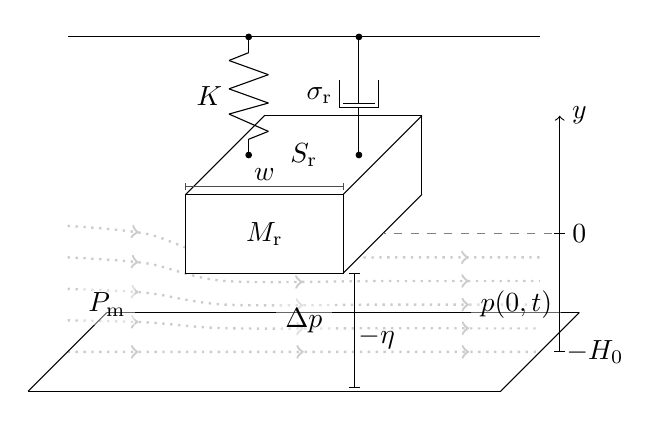
\begin{tikzpicture}
    
    \def\radius{6}; % Radius of the string (>2!)
    \pgfmathsetmacro{\reps}{3}; % How may back-and-forths in the drawing of the springs
    \def\bowSpacing{0.2};
    \def\drawingSpacing{1.5}
    \def\bowWidth{5};
    
    \def\woodWidth{1}; %>0.3
    \def\massWidth{2};
    \def\bridgeHeight{3};
    \def\bridgeWidth{4};
    \def\cornerRadius{0.15};
    \def\stringWidth{0.2};
    \pgfmathsetmacro{\tinyRadius}{\stringWidth*0.1};
    \pgfmathsetmacro{\stringWidthMinTinyRad}{((\stringWidth-(2*\tinyRadius)))*0.5};
    
    \def\axisLineWidth{0.07};

    % draw airflow
    
    %draw airflow
    \def\rightAirFlow{0}; % have the right airflow bulge (1) or not (0)
    \foreach \idx in {1,...,5}
    {
        \pgfmathsetmacro{\scaleLeft}{0.5 - 0.1 * \idx};
        \ifnum\rightAirFlow=1
            \pgfmathsetmacro{\scaleRight}{0.5 - 0.1 * \idx};
        \else
            \pgfmathsetmacro{\scaleRight}{0};
        \fi
        \begin{scope}[decoration={
            markings,
            mark=between positions 0.15 and 0.85 step 0.35
         with {\arrow{>}}}
            ]
        % \node at (0, \idx) {\scale};
         \draw [gray!40, 
         xshift=-2.5cm, 
         yshift= -\idx * 0.3cm, 
         dotted, 
         line width=0.3mm, postaction={decorate}] plot [smooth, tension = 0.5] coordinates { (0,1*\scaleLeft) (1,0.75*\scaleLeft) (2,0) (4, 0) (5, 0.75*\scaleRight) (6,1*\scaleRight)} ;
         \end{scope}
    }
    % \def\scale{0.5};
    % \draw [gray, xshift=-2.5cm, yshift=-0cm] plot [smooth, tension = 0.5] coordinates { (0,1*\scale) (1,0.75*\scale) (2,0) (4, 0) (5, 0.75*\scale) (6,1*\scale)};
    % \def\scale{0.25};
    % \draw [gray, xshift=-2.5cm, yshift=-1.2cm] plot [smooth, tension = 0.5] coordinates { (0,1*\scale) (1,0.75*\scale) (2,0) (4, 0) (5, 0.75*\scale) (6,1*\scale)};
    % \def\scale{0};
    % \draw [gray, xshift=-2.5cm, yshift=-1.5cm] plot [smooth, tension = 0.5] coordinates { (0,1*\scale) (1,0.75*\scale) (2,0) (4, 0) (5, 0.75*\scale) (6,1*\scale)};
    
    \node (r0) at ( 1.0,  -0.5 ) {}; % root
    \node (s0) at ( 1.0, 0.1 ) {}; % extreme
    \node (s1) at ( 1.6, 0.1 ) {}; % extreme

    % DRAW TREE
    \fill[fill=white] (r0.center)--(s0.center)--(s1.center);
    
    % \draw plot [smooth] coordinates {(-3, -3) (-2, 2) (-1, -3};
    \node at (0,0) [rectangle,draw, fill = white, minimum height=1cm,minimum width= \massWidth cm] (Mr) {$M_\text{r}$};
    %top
    % \draw[-] (-3, 2) -- (3, 2) node[below, midway] (top) {};
    % \draw[-] (-2, 3) -- (4, 3) node[below, midway] (top) {};
    % \draw[-] (-3, 2) -- (-2, 3) node[below, midway] (top) {};
    % \draw[-] (4, 3) -- (3, 2) node[below, midway] (top) {};
    \draw[-] (-2.5, 2.5) -- (3.5, 2.5) node[below, midway] (top) {};
    %bottom
    \draw[-] (-3, -2) -- (3, -2) node[below, midway] (bottom) {};
    \draw[-] (-2, -1) -- (4, -1) node[below, midway] (bottom) {};
    \draw[-] (-3, -2) -- (-2, -1) node[below, midway] (top) {};
    \draw[-] (4, -1) -- (3, -2) node[below, midway] (top) {};

    % draw mass
    
    \draw[-] (-1, 0.5) -- (0, 1.5) node[] (left) {};

    \draw[-] (1, 0.5) -- (2, 1.5) node[] (topRight) {};

    \draw[-] (0, 1.5) -- (2, 1.5) node[] (top) {};

    \draw[-] (2, 1.5) -- (2, 0.5) node[] (right) {};

    \draw[-] (0.5 * \massWidth, -0.5) -- (2, 0.5) node[] (bottomRight) {};

    \node[rotate = 0] at (0.5, 1) (Sr) {$S_\text{r}$};

    % eta line
    \draw[-, color = black] (0.5*\massWidth+2*\axisLineWidth, -0.5) -- (0.5*\massWidth+2*\axisLineWidth, -1.95)
    node[anchor = west] at (0.5*\massWidth +0.07, -1.33) (eta) {$-\eta$};

    \draw[-] (0.5 * \massWidth + \axisLineWidth, -0.5) -- (0.5 * \massWidth + 3*\axisLineWidth, -0.5) {}; 
    
    \draw[-] (0.5 * \massWidth +\axisLineWidth, -1.95) -- (0.5 * \massWidth +3*\axisLineWidth, -1.95); 
    \def\xOffset{0.3};
    % draw spring
    \filldraw[black] (-0.5 + \xOffset, 2.5) circle (1pt) node[anchor=center](topSpring){};    
    \draw[-] (-0.5 + \xOffset, 2.5) -- (-0.5 + \xOffset, 2.3);
    \draw[-] (-0.5 + \xOffset, 2.3) -- (-0.75 + \xOffset, 2.2);
    %switched these around because of the color
    \draw[-] (-0.25 + \xOffset, 2.02) -- (-0.75 + \xOffset, 1.84);
    \draw[-] (-0.75 + \xOffset, 2.2) -- (-0.25 + \xOffset, 2.02);
    \draw[-] (-0.75 + \xOffset, 1.84) -- (-0.25 + \xOffset, 1.66);
    \draw[-] (-0.25 + \xOffset, 1.66) -- (-0.75 + \xOffset, 1.52);
    \draw[-] (-0.75 + \xOffset, 1.52) -- (-0.25 + \xOffset, 1.3);
    \draw[-] (-0.25 + \xOffset, 1.3) -- (-0.5 + \xOffset, 1.2);
    \draw[-] (-0.5 + \xOffset, 1.2) -- (-0.5 + \xOffset, 1.0);
    \filldraw[black] (-0.5 + \xOffset, 1.0) circle (1pt) node[anchor=center](bottomSpring){};    
    \node at (-1 + \xOffset, 1.75) (K) {$K$};
    
    \def\dashpotHeight{-0.25}
    % draw dashpot
    \filldraw[black] (1.5 - \xOffset, 2.5) circle (1pt) node[anchor=center](topDashPot){};
    \draw[-] (1.5 - \xOffset, 2.5) -- (1.5 - \xOffset, 1.4 - \dashpotHeight);

    \draw[-] (1.3 - \xOffset, 1.4 - \dashpotHeight) -- (1.7 - \xOffset, 1.4 - \dashpotHeight);

    \draw[-] (1.25 - \xOffset, 1.7 - \dashpotHeight) -- (1.25 - \xOffset, 1.35 - \dashpotHeight);
    \draw[-] (1.75 - \xOffset, 1.35 - \dashpotHeight) -- (1.75 - \xOffset, 1.7 - \dashpotHeight);

    \draw[-] (1.25 - \xOffset, 1.35 - \dashpotHeight) -- (1.75 - \xOffset, 1.35 - \dashpotHeight);
    \draw[-] (1.5 - \xOffset, 1.35 - \dashpotHeight) -- (1.5 - \xOffset, 1.0);

    \filldraw[black] (1.5 - \xOffset, 1.0) circle (1pt) node[anchor=center](bottomDashpot){};    
    \node at (1.0 - \xOffset, 1.75) (sigma) {$\sigma_\text{r}$};
    
    
    % pressure labels
    \def\pressOffset{0.3}
    \def\backgroundOpacity{0.4}
    \node[fill = white, fill opacity=\backgroundOpacity, text opacity = 1] at (-2, -0.6 - \pressOffset) (Pm) {$P_\text{m}$};
    \node[fill = white, fill opacity=\backgroundOpacity, text opacity = 1] at (0.5, -0.8 - \pressOffset) (deltaP) {$\Delta p$};
    \node[fill = white, fill opacity=\backgroundOpacity, text opacity = 1] at (3.2, -0.6 - \pressOffset) (p) {$p(0,t)$};

    
    % y and H0
    \draw[dashed, color = gray] (3.65, 0) -- (1.5, 0);
    \node at (4, 1.5) {$y$};
    
    \draw[->] (3.75, -1.5) -- (3.75, 1.5);
    \node at (4, 0) {$0$};
    \draw (3.75 - \axisLineWidth, 0) -- (3.75 + \axisLineWidth, 0) {};


    \draw (3.75 - \axisLineWidth, -1.5) -- (3.75 + \axisLineWidth, -1.5) {};
    \node at (4.2, -1.5) {$-H_0$};
    
    % width
    \draw[black!70] (-1, 0.6) -- (1, 0.6) {};
    \draw[black!70] (-1, 0.55) -- (-1, 0.65) {};
    \draw[black!70] (1, 0.55) -- (1, 0.65) {};
    \node at (0, 0.75) (w) {$w$};
% \begin{scope}[very thick,decoration={
%     markings,
%     mark=at position 0.5 with {\arrow{>}}}
%     ] 
%     \draw[postaction={decorate}] (-4,0)--(4,0);
% \end{scope}
    
    \end{tikzpicture}
    \caption{Lipsystem with the equilibrium at 0 and the distance from the lower lip $H_0$. The various symbols relate to those used in Eq. \eqref{eq:lipReedCont}.}
    \label{fig:lipSystem}
\end{figure}

\subsection{Radiation}
As the bell-end of brass instruments is in a way ``coupled" to the air, the tube loses energy at the bell, or right boundary. These losses can be modelled using a radiation model and lossless condition \eqref{eq:contDirichlet} can be modified to be radiating instead. The radiation model used is the one for the unflanged cylindrical pipe proposed by Levine and Schwinger in \cite{Levine1948} and discretised by Silva \emph{et al.} in \cite{Silva2009}. As this model is not important for the contribution of this work it will not be detailed here in full. The interested reader is instead referred to \cite{Harrison2018} for a comprehensive explanation. 
  \section{Discretisation}\label{sec:discrete}
The continuous system described in the previous section is discretised using FDTD methods, which subdivide continuous equations into discrete points in space and time. Before moving on to this discretisation, we briefly introduce these methods along with several finite-difference operators.

\subsection{Numerical Methods}\label{sec:numMeth}
Consider a 1D system described by state variable $u = u(x,t)$ with spatial domain $x\in \mathbb{R}$ and time $t\geq 0$. The spatial domain can be disctretised according to $x=lh$ with spatial index $l \in \mathbb{Z}$ and grid spacing $h$ (in m) and time as $t=nk$ with temporal index $n \in \mathbb{Z}^{0+}$ and time step $k$ (in s). Using these discrete variables state variable $u(x,t)$ can be discretised to grid function $u_l^n$. 

Shift operators can then be applied to grid function $u_l^n$. Temporal and spatial shift operators are
\begin{equation}
    \begin{aligned}
        e_{t+}u_l^n &= u_l^{n+1}, \quad e_{t-}u_l^n = u_l^{n-1},\\
        e_{x+}u_l^n &= u_{l+1}^n\;, \quad \!e_{x-}u_l^n = u_{l-1}^n,
    \end{aligned}
\end{equation}
from which more complex operators can be derived.
First-order derivatives can be approximated using forward, backward and centred difference operators in time
\begin{equation}\label{eq:discTimeOperators}
    \delta_{t+} = \frac{e_{t+} - 1}{k},\ \delta_{t-} = \frac{1 - e_{t-}}{k},\ \delta_{t\cdot} = \frac{e_{t+}-e_{t-}}{2k},
\end{equation}
(all approximating $\partial_t$) and space
\begin{equation}\label{eq:discSpaceOperators}
    \delta_{x+} = \frac{e_{x+} - 1}{h},\ \delta_{x-} = \frac{1 - e_{x-}}{h},\ \delta_{x\cdot} = \frac{e_{x+}-e_{x-}}{2h},
\end{equation} 
(all approximating $\partial_x$) where the identity operator $1$ does not introduce any shift.

Furthermore, forward, backward and centred averaging operators can be defined in time
\begin{equation}
    \mu_{t+} = \frac{e_{t+} + 1}{2}, \ \mu_{t-} = \frac{1 + e_{t-}}{2}, \ \mu_{t\cdot} = \frac{e_{t+}+e_{t-}}{2},
\end{equation}
and space
\begin{equation}
    \mu_{x+} = \frac{e_{x+} + 1}{2}, \ \mu_{x-} = \frac{1 + e_{x-}}{2}, \ \mu_{x\cdot} = \frac{e_{x+}+e_{x-}}{2}.
\end{equation}
Here, forward and backward averaging operators are extremely useful in the context of first-order systems as used in this paper. When applied to a grid function, the result may be interpreted as its value shifted by half a temporal or spatial step: 
\begin{align}
    \mu_{t+}u_l^n &= u_l^{n+1/2}, \quad \mu_{t-}u_l^n = u_l^{n-1/2},\\
    \mu_{x+}u_l^n &= u_{l+1/2}^n, \quad \mu_{x-}u_l^n = u_{l-1/2}^n,
\end{align}
effectively placing the grid function on an \textit{interleaved grid} which will be further elaborated on in the following. 

\subsection{Discrete Tube}\label{sec:discSyst}
We start discretising system \eqref{eq:firstOrderSystem} by placing velocity $v$ on an interleaved grid, following \cite{Harrison2018}, both in space and time. Domain $x\in [0, L]$ can be discretised to $l = [0, \hdots, N]$ where number of intervals between grid points is calculated using \SWcomment[(same issue here as in the other paper)]
\begin{equation}\label{eq:numberOfIntervals}
    N=\lfloor L/h\rfloor.
\end{equation}

The grid functions $p_l^n \approx p(x,t)$ and $v_{l+1/2}^{n+1/2} \approx v(x,t)$ (with reduced domain $l = [0, \hdots, N-1]$) with $N+1$ and $N$ grid points respectively are then introduced along with discrete cross-sectional area $S_l\approx S(x)$ sampled at $x = lh$ to which the spatial operators defined in Section \ref{sec:numMeth} can also be applied.

System \eqref{eq:firstOrderSystem} can then be discretised into the following system of FDSs
\begin{subequations}\label{eq:FDS}
    \begin{align}
        \frac{\bar S_l}{\rho_0 c^2}\delta_{t+}p_l^n &= -\delta_{x-}(S_{l+1/2}v_{l+1/2}^{n+1/2}),\label{eq:discPressure}\\
        \rho_0 \delta_{t-}v_{l+1/2}^{n+1/2}&=-\delta_{x+}p_l^n,\label{eq:discVelocity}
    \end{align}
\end{subequations}
where $S_{l+1/2} = \mu_{x+}S_l$ and $\bar S_l = \mu_{x-}S_{l+1/2}$ are approximations to the continuous cross-sectional area $S(x)$. The values for $\bar S_l$ at the boundaries, i.e., $\bar S_0$ and $\bar S_N$ are set equal to $S(0)$ and $S(L)$.

Expanding the operators, we obtain the following recursion
\begin{subequations}\label{eq:updateNormal}
    \begin{align}
        p_l^{n+1} &= p_l^n - \frac{\rho_0 c \lambda}{\bar{S}_l}(S_{l+1/2}v_{l+1/2}^{n+1/2}-S_{l-1/2}v_{l-1/2}^{n+1/2}),\label{eq:pressureUpdate}\\
        v_{l+1/2}^{n+1/2} &= v_{l+1/2}^{n-1/2}-\frac{\lambda}{\rho_0 c}(p_{l+1}^n - p_l^n),\label{eq:velocityUpdate}
    \end{align}
\end{subequations}
where $\lambda = ck/h$ is referred to as the Courant number and
\begin{equation}\label{eq:CFL}
    \lambda \leq 1
\end{equation}
in order for the scheme to be stable. 

Finally, the boundary conditions in \eqref{eq:contBound} can be discretised as
\begin{subequations}
    \begin{align}
        \mu_{x-}\left(S_{1/2}v_{1/2}^{n+1/2}\right) = 0\label{eq:discNeumann}\\
        p_N^n = 0\label{eq:discDirich}
    \end{align}    
\end{subequations}

\subsection{Lip reed}
As the lip reed interacts with the particle velocity of the tube, it is placed on the interleaved temporal grid, but kept on the regular spatial grid, as it interacts with the boundary at $l=0$.

Equations \eqref{eq:lipReedCont} - \eqref{eq:lipBoundary} are discretised as follows:
\def\nphSys{n+1/2}
\begin{subequations}\label{eq:discreteLipSystem}
    \begin{align}
    &\begin{aligned}
        M_\text{r}\delta_{tt}y^{\nphSys} =&-M_\text{r}\omega_0^2\mu_{t\cdot}y^{\nphSys} -M_\text{r}\sigma_\text{r}\delta_{t\cdot}y^{\nphSys}\\
        &+\left(\mu_{t+}\psi^n\right)g^{n+1/2}+S_\text{r}\Delta p^{\nphSys},
    \end{aligned}\label{eq:discReed}\\
    &\Delta p^{\nphSys} = P_\text{m} - \mu_{t+}p_0^n,\label{eq:pDiff}\\
    &\begin{aligned}
        U_\text{B}^{\nphSys} =&\ w_\text{r}[-\eta^{\nphSys}]_+\text{sgn}(\Delta p^{\nphSys})\label{eq:bernoulli}\\
        &
        \cdot\sqrt{2|\Delta p^{\nphSys}|/\rho_0},
    \end{aligned}\\
    &U_\text{r}^{\nphSys}= S_\text{r}\delta_{t\cdot}y^{\nphSys},\label{eq:Ur}\\
    &\mu_{x-}(S_{1/2}v_{1/2}^{\nphSys})= U_\text{B}^{\nphSys} + U_\text{r}^{\nphSys},\label{eq:UbUr}
    \end{align}
\end{subequations}
where $\omega_0 = \omega_0^{n+1/2}$ and $P_\text{m} = P_\text{m}^{n+1/2}$ and
\begin{subnumcases}{ \label{eq:gDef} g^{n+1/2} =}
\begin{aligned}
\kappa&\sqrt{\frac{K_\text{c}(\alpha+1)}{2}}\\
&\cdot(\eta^{n+1/2})^{\frac{\alpha-1}{2}}
\end{aligned} & if $\eta^{n+1/2} \geq 0$ \label{eq:collCorr1}\\
-2 \frac{\psi^n}{\eta^\star-\eta^{n-1/2}} & if $\eta^{n+1/2} < 0$ \label{eq:collCorr2}
\end{subnumcases}
and $\kappa = 1$ if $\psi^n \geq 0$, otherwise $\kappa = -1$. Finally, $\eta^\star = -y^{\star} - H_0$ where $y^{\star}$ is the value of $y^{n+3/2}$ calculated using system \eqref{eq:discreteLipSystem} (after expansion) without the collision potential. This means that system \eqref{eq:discreteLipSystem} needs to be calculated twice every iteration, once without the collision term and once with. The process of calculating the pressure difference $\Delta p^{n+1/2}$ in \eqref{eq:discreteLipSystem} will not be given here, but the interested reader is referred to \cite[Ch. 5]{Harrison2018} for a derivation.

Finally, to couple the lip reed to the tube, boundary condition \eqref{eq:discNeumann} can be modified to Eq. \eqref{eq:UbUr}. 
% \begin{subnumcases}{\label{eq:discreteLipSystem}}
%     M_\text{r}\delta_{tt}y^{\nphSys} = -M_\text{r}\omega_0^2\mu_{t\cdot}y^{\nphSys} -M_\text{r}\sigma_\text{r}\delta_{t\cdot}y^{\nphSys}\label{eq:discReed}\\\qquad \qquad \qquad \ \ \ 
%     +\ S_\text{r}\Delta p^{\nphSys}\nonumber\\
%     \Delta p^{\nphSys} = P_\text{m} - \mu_{t+}p_0^n\label{eq:pDiff}\\
%     U_\text{B}^{\nphSys} = w[y^{\nphSys}+H_0]_+\text{sgn}(\Delta p^{\nphSys})\label{eq:bernoulli}\\\qquad \qquad \ \ \ 
%     \cdot\ \sqrt{2|\Delta p^{\nphSys}|/\rho_0}\nonumber\\
%     U_\text{r}^{\nphSys}= S_\text{r}\delta_{t\cdot}y^{\nphSys}\label{eq:Ur}\\
%     \mu_{x-}(S_{1/2}v_{1/2}^{\nphSys})= U_\text{B}^{\nphSys} + U_\text{r}^{\nphSys}\label{eq:UbUr}
% \end{subnumcases}

% \begin{subnumcases}{\label{eq:discreteLipSystem}}
%     M_\text{r}\delta_{tt}y^{\nphSys} & $= -M_\text{r}\omega_0^2\mu_{t\cdot}y^{\nphSys}-M_\text{r}\sigma_\text{r}\delta_{t\cdot}y^{\nphSys} + S_\text{r}\Delta p^{\nphSys}$\label{eq:discReed}\\
%     \Delta p^{\nphSys} & $= P_\text{m} - \mu_{t+}p_0^n$\label{eq:pDiff}\\
%     U_\text{B}^{\nphSys} & $= w[y^{\nphSys}+H_0]_+\text{sgn}(\Delta p^{\nphSys})\sqrt{\frac{2|\Delta p^{\nphSys}|}{\rho_0}}$\label{eq:bernoulli}\\
%     U_\text{r}^{\nphSys} & $= S_\text{r}\delta_{t\cdot}y^{\nphSys}$\label{eq:Ur}\\
%     \mu_{x-}(S_{1/2}v_{1/2}^{\nphSys})\!\!\!\!\! \!\!\!\!\! &$= U_\text{B}^{\nphSys} + U_\text{r}^{\nphSys}$\label{eq:UbUr}
% \end{subnumcases}
  \begin{figure*}[t]
    \centering
    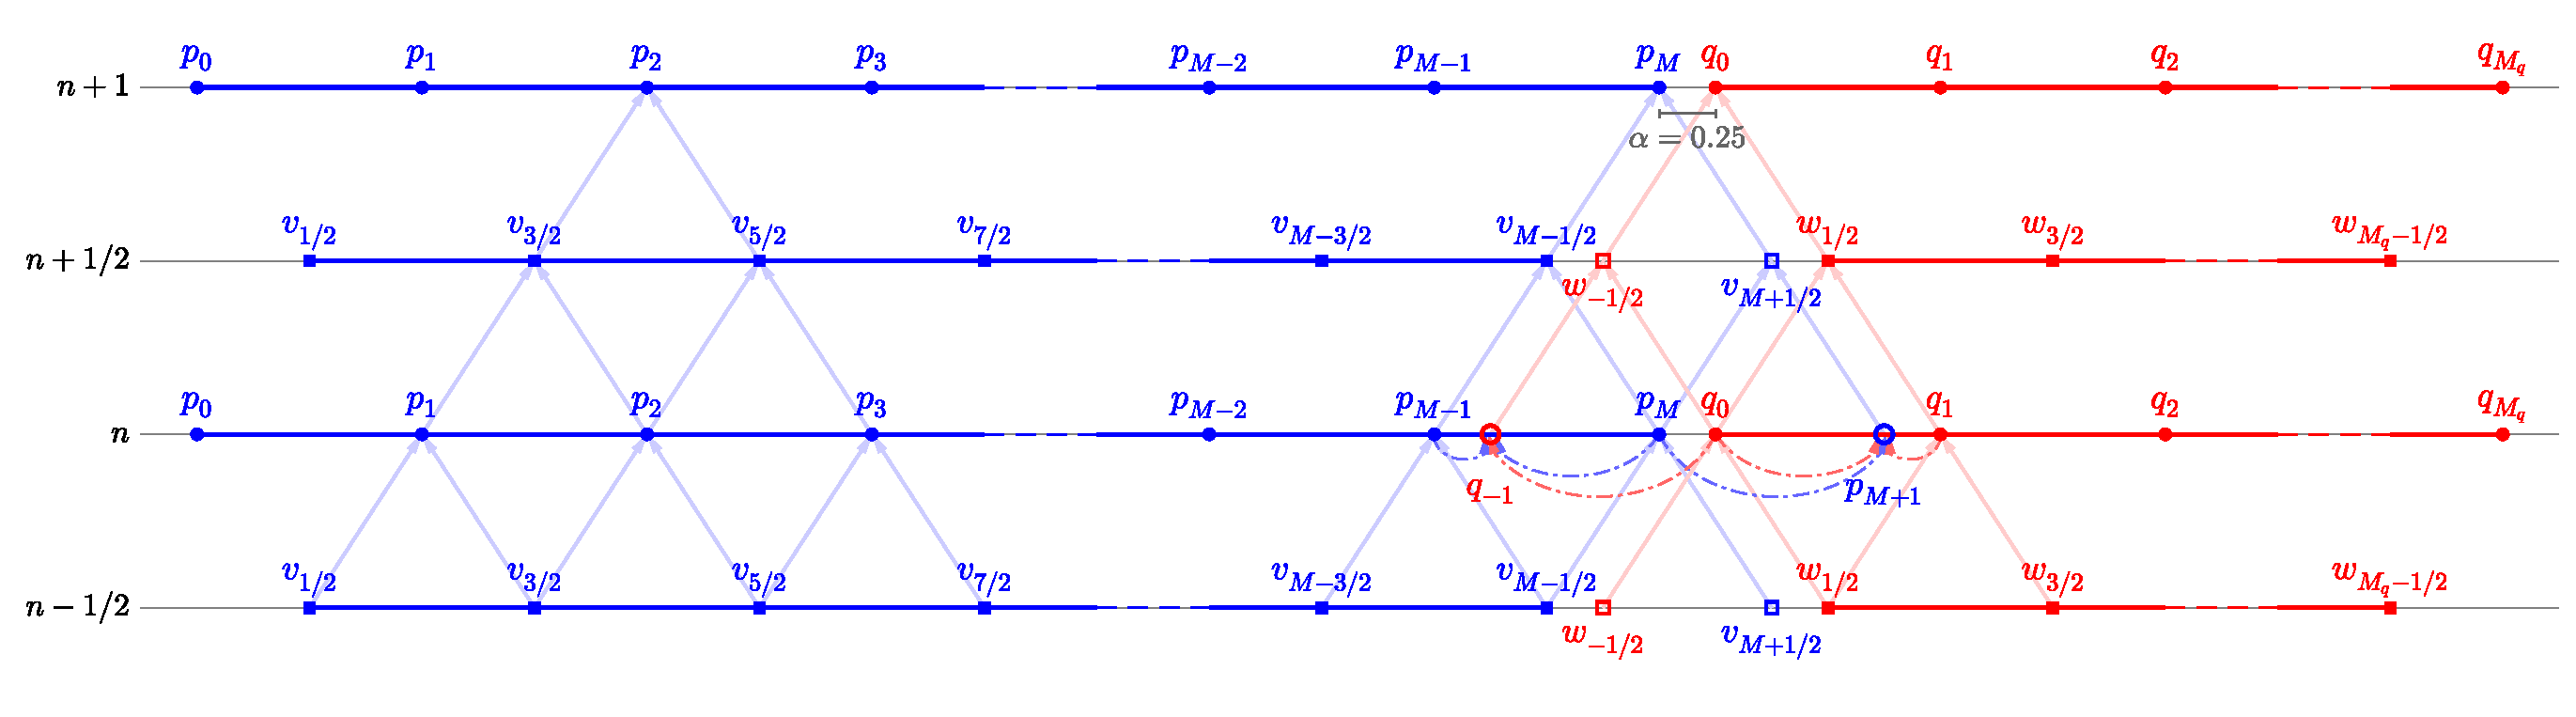
\includegraphics[width = \textwidth]{Figures/tromboneSchematic.eps}
    \caption{Schematic showing data flow of how different grid points at time index $n+1$ are calculated with $\alpha = 0.25$ in Eq. \eqref{eq:alphaDef}. To prevent cluttering, arrows going straight up (indicating that the state of a grid point at time step $n$ is needed to calculate the state of that grid point at $n+1$) are suppressed. As an example of the usual case, the points required to calculate $p_2^{n+1}$ are shown (refer to Eq. \eqref{eq:updateNormal}). Furthermore, the points needed to calculate $p_{M}^{n+1}$ and $q_0^{n+1}$ are shown. The most important difference with the usual case is that the virtual grid points $p_{M_p+1}^n$ and $q_{-1}^n$ 
    are the result of the interpolation of known pressure values at $n$ using Eq. \eqref{eq:connectionInterpol}. %and velocity values at $n+1/2$ respectively
    %
    %\SWcomment[Seemingly, $q_0^n$ is not calculated from anything, but it is simply $q_0^{n+1}$ time-shifted back. The same would be shown for $v_{M_p+1/2}^{n-1/2}$, but the figure does not go back-in-time more than this.]
    \label{fig:dynamicGridSchematic}}
\end{figure*}

\section{Dynamic grid}\label{sec:dynamicGrid}
Arguably the most characteristic feature of the trombone is its slide with which the length of the tube is altered and the resonating frequencies are changed. In a companion article \cite{Willemsen2021}, we present a method to dynamically change grid configurations of FDSs by adding and subtracting grid points based on paramters describing the system. Though \cite{Willemsen2021} shows changes in the wavespeed $c$ rather than the length $L$, the effect of a change in either of these parameters has an identical effect on these systems \SWcomment[as long as the geometry is unchanged for the grid points.] Leaving $c$ fixed also means that grid spacing $h$ does not change during the simulation, but rather the spatial domain of the system. Note that this method only works for slow (sub-audio rate) parameter changes.

We can split a tube with time-varying length $L^n$ into two smaller sections with lengths $L_p^n$ and $L_q^n$ (in m) such that $L^n = L_p^n + L_q^n$. Splitting the FDSs in \eqref{eq:FDS} in this way yields two sets of first-order systems. The pressure and particle velocity of the first (left) system $p_\lp^n$ and $v_{\lp+1/2}^{n+1/2}$ are both defined over discrete domain $\lp = [0, \hdots, M^n]$, and those of the second (right) system $q_\lq^n$ and $w_{\lq-1/2}^{n+1/2}$ are defined over discrete domain $\lq = [0, \hdots, M_q^n]$, with
\begin{equation}\label{eq:MMq}
    M^n = \lceil L_p^n/h\rceil, \quad \text{and} \quad M_q^n = \lfloor L_q^n/h\rfloor
\end{equation} where $\lceil \cdot \rceil$ and $\lfloor \cdot \rfloor$ denote the ceiling and flooring operation respectively. Note, that the domains for $v$ and $w$ have an extra grid point when compared to the regular case in \eqref{eq:FDS} and that $w$ is indexed with $\lq-1/2$ rather than $\lq+1/2$. The resulting system of FDSs then becomes
\begin{subequations}\label{eq:firstOrderPairs}
    \begin{align}
        \frac{\bar S_\lg}{\rho_0 c^2}\delta_{t+}p_\lp^n &= -\delta_{x-}(S_{\lg+1/2}v_{\lp+1/2}^{n+1/2}),\label{eq:discPressureP}\\
        \rho_0 \delta_{t-}v_{\lp+1/2}^{n+1/2}&=-\delta_{x+}p_\lp^n,\label{eq:discVelocityV}\\
        \frac{\bar S_\lg}{\rho_0 c^2}\delta_{t+}q_\lq^n &= -\delta_{x+}(S_{\lg-1/2}w_{\lq-1/2}^{n+1/2}),\label{eq:discPressureQ}\\
        \rho_0 \delta_{t-}w_{\lq-1/2}^{n+1/2}&=-\delta_{x-}q_\lq^n.\label{eq:discVelocityW}
    \end{align}
\end{subequations}
Here, due to the different indexing for $w$, the spatial derivatives for the right system are flipped. Also note, that $l$ is still used for the spatial indices of $\bar S$ and $S$, where $l\in [\lp, \lq+M^n]$. The conditions for the outer boundaries of this system, i.e., at $\lp = 0$ and $\lq = M_q^n$, are the same as for the full system. The inner boundaries, $\lp = M^n$ and $\lq = 0$ are connected according to the method described in \cite{Willemsen2021} which will be explained shortly.
To be able to calculate $p_M^{n+1}$ and $q_0^{n+1}$, the domains of $v$ and $w$ have been extended at the inner boundaries to include $v_{M+1/2}^{n+1/2}$ and $w_{-1/2}^{n+1/2}$. These, however, need points outside of the domains of $p_\lp^n$ and $q_\lq^n$, i.e., $p_{M+1}^n$ and $q_{-1}^n$. In \cite{Willemsen2021} we propose to calculate these \textit{virtual grid points} based on known values of the system. Despite the fact that \cite{Willemsen2021} presents the method using a second-order system, it can still be applied here. The process of how the $p_M^{n+1}$ and $q_0^{n+1}$ are calculated is visualised in in Figure \ref{fig:dynamicGridSchematic}.

\subsection{Changing the Tube Length}
In the following, the location of a grid point $u_l$ along the grid (in m from the left boundary) from is denoted as $x_{u_l}$.

The two pairs of first order systems in \eqref{eq:firstOrderPairs} are placed on the same domain $x$ with
\begin{equation}\label{eq:gridLocations}
    x_{p_\lp} = \lp h, \quad \text{and}\quad
    x_{q_\lq} = L^n-(M_q^n - \lq)h
\end{equation}
describing the locations of the left system and right system respectively. It can be observed from Eq. \eqref{eq:gridLocations} that as the tube length $L^n$ changes, the locations of the grid points of the right system will change. More specifically, as the trombone-slide is extended and $L^n$ increases, all grid points of the right system move to the right, and vice versa for a contracting slide. If $L^n$ is changed in a smooth fashion, the continuous domain $x \in [0,L^n]$ will not necessarily be subdivided into an integer amount of intervals $N^n$ (of size $h$). This is where a \textit{fractional} number of intervals is introduced and is defined as 
\begin{equation}\label{eq:nfrac}
    \Nfrac^n = L^n/h,
\end{equation}
which is essentially Eq. \eqref{eq:numberOfIntervals} without the flooring operation, and $N^n = \lfloor \Nfrac^n \rfloor$. The fractional part of $\Nfrac^n$ can then be calculated using
\begin{equation}\label{eq:alphaDef}
    \alpha = \alpha^n = \Nfrac^n - N^n,
\end{equation}
which describes the distance between the inner boundaries along the grid in terms of how many times $h$ would fit in-between (which is always less than once). If $\Nfrac^n = N^n$ and $\alpha = 0$, the inner boundaries $p_M$ and $q_0$ perfectly overlap, i.e., $x_{p_M}^n = x_{q_0}^n$. This also means that the domain $x$ can be exactly divided into $N^n$ equal intervals of size $h$. As the virtual grid points $p_{M+1}^n$ and $q_{-1}^n$ perfectly overlap with $q_{1}^n$ and $p_{M-1}^n$ respectively, these values can be used directly to calculate the inner boundaries. This situation effectively acts as a rigid connection between the inner boundaries defined as
\begin{equation}\label{eq:rigidConn}
    p_M^n = q_0^n.
\end{equation}
%
If $\alpha \neq 0$, some other definition for $p_{M+1}^n$ and $q_{-1}^n$ needs to be found. We use quadratic Lagrangian interpolation according to
\begin{subequations}\label{eq:connectionInterpol}
\begin{align}
        &p_{M+1}^n = \frac{\alpha - 1}{\alpha + 1}p_{M}^n + q_0^n - \frac{\alpha - 1}{\alpha + 1}q_1^n
    \label{eq:calcPMp1}\\
        &q_{-1}^n
        =-\frac{\alpha - 1}{\alpha + 1}p_{M-1}^n + p_{M}^n+ \frac{\alpha - 1}{\alpha + 1}q_{0}^n.\label{eq:calcQm1}
\end{align}
\end{subequations}
which can then be used to calculate $v_{M+1/2}^{n+1/2}$ and $w_{-1/2}^{n+1/2}$ and consequently $p_M^{n+1}$ and $q_0^{n+1}$. This process repeats every sample. It can be shown through the rigid connection in \eqref{eq:rigidConn}, that if $\alpha=0$, the definitions in \eqref{eq:connectionInterpol} reduce to $p_{M+1}^n = q_1^n$ and $q_{-1}^n = p_{M-1}^n$ as stated before.

\subsection{Adding and removing grid points}\label{sec:addRemove}
As the tube length $L^n$ changes, $L_p^n$ and $L_q^n$ also change according to
\begin{equation}
    L_p^n = L_p^{n-1} + 0.5 L_\text{diff}^n, \quad L_q^n =  L_q^{n-1} + 0.5L_\text{diff}^n,\label{eq:updateLs} 
\end{equation}
where
\begin{equation}
    L_\text{diff}^n = L^n-L^{n-1},\label{eq:lDiff}
\end{equation}
which causes the number of points $M^n$ and $M_q^n$ to change as well according to Eq. \eqref{eq:MMq}. The following state vectors are introduced for the pressure, defined for $n+1$ and $n$ 
\begin{equation}
    \mathbf{p}^n = [p_0^n, p_1^n, ..., p_M^n]^T,\ \mathbf{q}^n = [q_0^n, q_1^n, ..., q_{M_q}^n]^T
\end{equation}
and for the velocity, defined for $n+1/2$ and $n-1/2$
\begin{equation}
    \begin{aligned}
        \mathbf{v}^{n-1/2} &=  [v_{1/2}^{n-1/2}, v_{3/2}^{n-1/2}, ..., v_{M+1/2}^{n-1/2}]^T\\
        \mathbf{w}^{n-1/2} &=  [w_{-1/2}^{n-1/2}, w_{1/2}^{n-1/2}, ..., w_{M_q-1/2}^{n-1/2}]^T
    \end{aligned}
\end{equation}
and contain the different states over the discrete domains defined at the beginning of this section. Here, $T$ denotes the transpose operation.

If $N^n>N^{n-1}$, points are added to the left and right system in an alternating fashion \SWcomment[($n-1$ is used later on for the state correction, say something about that here or leave for Section \ref{sec:impStateCorr}..?)]
\begin{equation}\label{eq:addingPoint}
    \begin{aligned}
        \!\!\!\!\!&\begin{cases}
            \mathbf{p}^n = [(\mathbf{p}^n)^T, I_3\mathbf{r}^n]^T\\
            \mathbf{v}^{n-1/2} = [(\mathbf{v}^{n-1/2})^T, I_3\mathbf{z}_v^{n-1/2}]^T
        \end{cases}
        \quad\!\text{if $N^n $ is odd},\\
        \!\!\!\!\!&\begin{cases}
            \mathbf{q}^n = [I_3^\flip\mathbf{r}^n, (\mathbf{q}^n)^T]^T\\
            \mathbf{w}^{n-1/2} = [ I_3^\flip\mathbf{z}_w^{n-1/2},(\mathbf{w}^{n-1/2})^T]^T
        \end{cases}\text{if $ N^n$ is even},
    \end{aligned}
\end{equation}
where
\begin{equation}\label{eq:interpVecs}
    \begin{aligned}
        \!\!\!\!\mathbf{r}^n &= [p_{M-1}^n, p_M^n, q_0^n, q_1^n]^T,\\
        \!\!\!\!\mathbf{z}_v^{n-1/2} &= [v_{M-1/2}^{n-1/2}, v_{M+1/2}^{n-1/2}, w_{1/2}^{n-1/2}, w_{3/2}^{n-1/2}]^T - \boldsymbol{\eta},\\
        \!\!\!\!\mathbf{z}_w^{n-1/2} &= [v_{M-3/2}^{n-1/2}, v_{M-1/2}^{n-1/2}, w_{-1/2}^{n-1/2}, w_{1/2}^{n-1/2}]^T+ \boldsymbol{\eta}^{\flip},% \quad\text{and}\\
        %     \mathbf{v}_\star^n &= [w_1^n, w_0^n, u_M^n, u_{M-1}^n],
    \end{aligned}
\end{equation}
cubic Lagrangian interpolator
\begin{equation}\label{eq:customIp}
    I_3 = \begin{bmatrix} -\frac{\alpha(\alpha+1)}{(\alpha+2)(\alpha+3)} &\frac{2\alpha}{\alpha+2} &\frac{2}{\alpha+2} 
    &-\frac{2\alpha}{(\alpha+3)(\alpha+2)}
    \end{bmatrix},
\end{equation}
and 
\begin{equation}\label{eq:offsetVec}
    \boldsymbol{\eta} = \boldsymbol{\eta}^{n-1/2}= \left(w_{-1/2}^{n-1/2}-v_{M+1/2}^{n
    -1/2}\right)\cdot[0, 0, 1, 1]^T 
\end{equation}
adds an offset to half of the $\mathbf{z}$ vectors depending on the state-difference between the inner boundaries of $v$ and $w$. This will be further explained in Section \ref{sec:drift}. Finally, $I_3^\flip$ and $\boldsymbol{\eta}^{\flip}$ are flipped versions of \eqref{eq:customIp} and \eqref{eq:offsetVec} respectively.

If $N^n < N^{n-1}$ points are simply removed from the vectors according to

\begin{equation}\label{eq:removingPoint}
    \begin{aligned}
        &\begin{cases}
            \mathbf{p}^n = [p_0^n, \hdots, p_{M-1}^n]^T\\
            \mathbf{v}^{n-1/2} = [v_{1/2}^{n-1/2}, \hdots, v_{M-1/2}^{n-1/2}]^T
        \end{cases}
        \quad\!\text{if $N^n $ is even},\\
        &\begin{cases}
            \mathbf{q}^n = [q_1^n, \hdots, q_{M_q}^n]^T\\
            \mathbf{w}^{n-1/2} = [w_{1/2}^{n-1/2},\hdots, w_{M_q-1/2}^{n-1/2}]^T
        \end{cases}\text{if $ N^n$ is odd},
    \end{aligned}
\end{equation}

\subsection{Drift of $w$}\label{sec:drift}
The inner boundaries of the pressure states $p$ and $q$ are connected by \eqref{eq:connectionInterpol}, but no such connection exists for the velocity states $v$ and $w$. As this leaves $w$ without any boundary condition (recall that the right boundary condition only exists for the pressure as in \eqref{eq:discDirich}) it is only ``held in place'' by the pressure values of $q$, or more specifically, by derivatives (both spatial and temporal). As the discretisation is an approximation, it does not give a perfect solution and $w$ tends to `drift' during the simulation, especially when $L^n$ is changed.

\SWcomment[Luckily], as the pressure values are also calculated from derivatives of the velocity, the absolute states of $v$ and $w$ do not matter. The difference in values at the connection point is also irrelevant as there is no spatial derivative taken between $v$ and $w$ (refer to Figure \ref{fig:dynamicGridSchematic}). Finally, the pressure values are used for the sound-output of the simulation, so the drift does not cause any audible artefacts. 

The absolute states do, however, need to be accounted for when adding points to the velocity vectors in \eqref{eq:addingPoint}. The current drift can be approximated by observing the difference between $w_{-1/2}^{n-1/2}$ and $v_{M+1/2}^{n-1/2}$, as these have approximately the same $x$ location ($x_{w_{-1/2}}^n \approx x_{v_{M+1/2}}^n$) when a grid point is added. This is then used in a drift-correction vector $\boldsymbol{\eta}^{n-1/2}$ presented in \eqref{eq:interpVecs}. When a point is added to $v$, the values of $w$ in $\mathbf{z}_{v}$ are offset by the aforementioned difference and when a point is added to $w$ the same happens (inverted) for the values of $v$ in $\mathbf{z}_w$. This way, the drift is allowed, but does not affect the state of the newly added grid points. Note that the drift does not affect the operations of point removal in \eqref{eq:removingPoint}.

\subsection{State Correction}
As $L^n$, and with that the number of grid points, is decreased, it might occur that the inner boundaries $p_M^n$ and $q_0^n$ have a very different value when $\alpha \gtrsim 0$, i.e., right before a point is removed. This violates the rigid connection in Eq. \eqref{eq:rigidConn}. 

We propose in \cite{Willemsen2021} to add an artificial spring-like connection between the inner boundaries that ``corrects'' the state of these points. Applying this to system \eqref{eq:firstOrderPairs} extends Eqs. \eqref{eq:discPressureP} and \eqref{eq:discPressureQ} according to
\begin{subequations}\label{eq:pressuresWithSC}
    \begin{align}
        \frac{\bar S_\lg}{\rho_0 c^2}\delta_{t+}p_\lp^n &= -\delta_{x-}(S_{\lg+1/2}v_{\lp+1/2}^{n+1/2}) + J_p(x_{p_M})F_\text{sc}\label{eq:pWithSC}\\
        \frac{\bar S_\lg}{\rho_0 c^2}\delta_{t+}q_\lq^n &= -\delta_{x+}(S_{\lg-1/2}w_{\lq-1/2}^{n+1/2}) - J_q(x_{q_0})F_\text{sc}\label{eq:qWithSC}
    \end{align}
\end{subequations}
where spreading operators
\begin{equation}\label{eq:spreadingOperators}
    \begin{aligned}
    J_p(x_i)& =
    \begin{cases}
        \frac{1}{h}, & \lp = \lp_{\!,i} = \lfloor x_i/h\rfloor\\
        0,& \text{otherwise},
    \end{cases}
    \quad\text{and}\\
    J_q(x_i) &=
    \begin{cases}
        \frac{1}{h}, & \lq = \lq_{\!,i} = \lfloor x_i/h \rfloor - M\\
        0,& \text{otherwise},
    \end{cases}
\end{aligned}
\end{equation}
correction effect
\begin{equation}\label{eq:scForce}
    F_\text{sc} = \beta\left(\omega_\text{sc}^2\mu_{t\cdot}\eta_\text{sc}^n+\sigma_\text{sc}\delta_{t\cdot}\eta_\text{sc}^n\right)
\end{equation}
(in m$^{3}$/s)\SWcomment[..units stop making sense here as this is an artificial connection ``force''.. might just exclude them?], with spring stiffness $\omega_\text{sc}$, spring damping $\sigma_\text{sc}$, pressure difference
\begin{equation}
    \eta_\text{sc}^n \triangleq q_0^n - p_M^n
\end{equation}
(in N/m$^2$) and scaling coefficient
\begin{equation}\label{eq:betaDef}
    \beta = \beta(\alpha) = \frac{1-\alpha}{\alpha+\epsilon},
\end{equation}
where $\epsilon\ll 1$ to prevent division by 0. Just like in \cite{Willemsen2021}, implementing the pressure difference allows for an infinite $\beta$ ($\epsilon = 0$) acting like a rigid connection between Eqs. \eqref{eq:pWithSC} and \eqref{eq:qWithSC}.

\SWcomment[Matrix form here??]

One can write the entire system above in matrix form by concatenating...

  \section{Implementation}

\subsection{Parameters}
A schematic showing the trombone geometry is shown in Figure \ref{fig:tromboneSchematic} and the lengths and radii used in Table \ref{tab:geometry}.

Other parameters used in the simulation can be found in Table \ref{tab:parameters}.


\begin{table}[t]
    \small
    \begin{center}
    \begin{tabular}{|l|c|c|}
        \hline
        Part of tube & Length (cm) & Radius (cm)\\\hline
        Inner slide (1) & 70.8 & 0.69\\
        Outer slide (extended) (2) & 53 & 0.72 
        \\
        Slide crook (3)& 17.7 & 0.74\\
        Outer slide (extended) (4) & 53 & 0.72 
        \\
        Inner slide (5) & 71.1 & 0.69\\
        Gooseneck (6) & 24.1 & 0.71\\
        Tuning slide (7) & 25.4 & 0.75, 1.07\\
        Bell flare (8) & 56.7 \SWcomment[$\leftarrow$check]& 1, 10.8\\\hline
    \end{tabular}
    \caption{Geometry of a measured trombone taken from \cite{Smyth2011}. Numbers correspond to Figure \ref{fig:tromboneSchematic}.\label{tab:geometry}}
    \end{center}
\end{table}

\begin{figure}[ht]
    \centering
    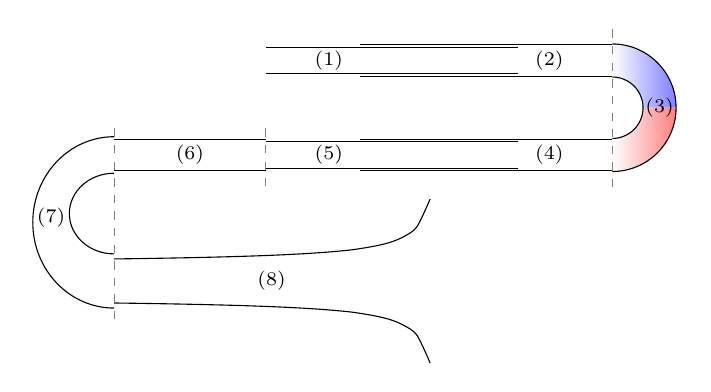
\begin{tikzpicture}[scale = 8]

    \def\labelColor{black};
    \def\labelSize{\fontsize{7pt}{7pt}\selectfont};

    \def\hornOffset{0.025};
    \def\stepSize{0.004}

    \def\dashedLineColor{gray};
    \def\dashedLineOvershoot{0.025}
    % tuning slide params
    \def\tuningSlideDim{0.1};
    \pgfmathsetmacro{\tuningSlideRad}{\stepSize + \hornOffset};
    \def\tuningSlideOffset{0.007};

    % gooseneck params
    \def\gooseNeckLength{0.241};
    \pgfmathsetmacro{\gooseNeckRad}{\tuningSlideRad - \stepSize};

    % inner slide params
    \def\innerLength{0.4};
    \pgfmathsetmacro{\innerRad}{\gooseNeckRad - \stepSize};

    % outer slide params
    \def\outerLength{\innerLength};
    \pgfmathsetmacro{\outerRad}{\gooseNeckRad};
    \pgfmathsetmacro{\extension}{0.15};

    \def\endOfSlideDim{0.075};
    \pgfmathsetmacro{\endOfSlideRad}{\outerRad * 1.05};

    %% draw horn

    \draw[domain=0:0.502, smooth, variable=\x, black] plot ({\x}, {\hornOffset + 0.0063 * ((0.502-\x) + 0.0174)^(-0.7)});
    
    \draw[domain=0:0.502, smooth, variable=\x, black] plot ({\x}, {-\hornOffset-0.0063 * ((0.502-\x) + 0.0174)^(-0.7)});
    
    \node[anchor = center, color = \labelColor](eight) at (0.25, 0) {\labelSize(8)};

    % draw tuningSlide
    \pgfmathsetmacro{\innerTuningSlideDim}{(\tuningSlideDim - \tuningSlideRad)}
    \pgfmathsetmacro{\outerTuningSlideDim}{(\tuningSlideDim + \tuningSlideRad)}

    \node[anchor = center, color = \labelColor](seven) at (-\innerTuningSlideDim-\tuningSlideRad, \innerTuningSlideDim+\tuningSlideRad) {\labelSize(7)};

    \pgfmathsetmacro{\innerTuningSlideWithOffset}{\innerTuningSlideDim - \tuningSlideOffset}

    \pgfmathsetmacro{\outerTuningSlideWithOffset}{\outerTuningSlideDim + \tuningSlideOffset}

    \draw (0, 2*\tuningSlideDim-\tuningSlideRad) arc(90:270:\innerTuningSlideDim cm and \innerTuningSlideWithOffset cm);

    \draw (0, 2*\tuningSlideDim+\tuningSlideRad) arc(90:270:\outerTuningSlideDim cm and \outerTuningSlideWithOffset cm);
    
    % dashedline
    \draw[dashed, color = \dashedLineColor] (0, -\tuningSlideRad-\tuningSlideOffset-\dashedLineOvershoot) -- (0, 2*\tuningSlideDim+\tuningSlideRad+\dashedLineOvershoot);

    % draw gooseneck
    \draw (0, 2*\tuningSlideDim + \gooseNeckRad) -- (\gooseNeckLength, 2*\tuningSlideDim + \gooseNeckRad);

    \draw (0, 2*\tuningSlideDim - \gooseNeckRad) -- (\gooseNeckLength, 2*\tuningSlideDim - \gooseNeckRad);

    \node[anchor = center, color = \labelColor](six) at (0.5 * \gooseNeckLength, 2*\tuningSlideDim) {\labelSize(6)};

    % dashedline
    \draw[dashed, color = \dashedLineColor] (\gooseNeckLength, 2*\tuningSlideDim-\gooseNeckRad-\dashedLineOvershoot) -- (\gooseNeckLength, 2*\tuningSlideDim+\gooseNeckRad+\dashedLineOvershoot);

    % draw inner slide
    \draw (\gooseNeckLength, 2*\tuningSlideDim + \innerRad) -- (\gooseNeckLength+\innerLength, 2*\tuningSlideDim + \innerRad);

    \draw (\gooseNeckLength, 2*\tuningSlideDim - \innerRad) -- (\gooseNeckLength+\innerLength, 2*\tuningSlideDim - \innerRad);

    \node[anchor = center, color = \labelColor](five) at (\gooseNeckLength + 0.25 * \innerLength, 2*\tuningSlideDim) {\labelSize(5)};

    % draw outer slide
    \pgfmathsetmacro{\outerSlideStart}{\gooseNeckLength + \extension};

    \draw (\outerSlideStart, 2*\tuningSlideDim + \outerRad) -- (\outerSlideStart+\outerLength, 2*\tuningSlideDim + \outerRad);

    \draw (\outerSlideStart, 2*\tuningSlideDim - \outerRad) -- (\outerSlideStart+\outerLength, 2*\tuningSlideDim - \outerRad);

    \node[anchor = center, color = \labelColor](four) at (\outerSlideStart + 0.75 * \outerLength, 2*\tuningSlideDim) {\labelSize(4)};


    % draw end of slide
    
    \pgfmathsetmacro{\innerEndOfSlideDim}{(\endOfSlideDim - \endOfSlideRad)};
    \pgfmathsetmacro{\outerEndOfSlideDim}{(\endOfSlideDim + \endOfSlideRad)};

    \pgfmathsetmacro{\startEndOfSlide}{\outerSlideStart + \outerLength};
    % division blue
    \fill[white, left color=white, right color=blue, fill opacity = 0.5] 
    (\startEndOfSlide+\innerEndOfSlideDim,2*\tuningSlideDim+\endOfSlideDim) 
    arc (0:90:\innerEndOfSlideDim cm and \innerEndOfSlideDim cm) 
    -- (\startEndOfSlide,2*\tuningSlideDim+\endOfSlideDim + \innerEndOfSlideDim)
    -- (\startEndOfSlide,2*\tuningSlideDim+2*\endOfSlideDim+\endOfSlideRad)
    arc (90:0:\outerEndOfSlideDim cm and \outerEndOfSlideDim cm)
    -- (\startEndOfSlide+\outerEndOfSlideDim,2*\tuningSlideDim+\endOfSlideDim)
    -- cycle;

    % division red
    \fill[white, left color=white, right color=red, fill opacity = 0.5] 
    (\startEndOfSlide+\innerEndOfSlideDim,2*\tuningSlideDim+\endOfSlideDim) 
    arc (0:-90:\innerEndOfSlideDim cm and \innerEndOfSlideDim cm) 
    -- (\startEndOfSlide,2*\tuningSlideDim+\endOfSlideDim)
    -- (\startEndOfSlide,2*\tuningSlideDim-\endOfSlideRad)
    arc (-90:0:\outerEndOfSlideDim cm and \outerEndOfSlideDim cm)
    -- (\startEndOfSlide+\outerEndOfSlideDim,2*\tuningSlideDim+\endOfSlideDim)
    -- cycle;

    \draw (\startEndOfSlide, 2*\tuningSlideDim+\endOfSlideRad) arc(-90:90:\innerEndOfSlideDim cm and \innerEndOfSlideDim cm);

    \draw (\startEndOfSlide, 2*\tuningSlideDim-\endOfSlideRad) arc(-90:90:\outerEndOfSlideDim cm and \outerEndOfSlideDim cm);

    \node[anchor = center, color = \labelColor](three) at (\startEndOfSlide + \innerEndOfSlideDim + \endOfSlideRad, 2*\tuningSlideDim+ \innerEndOfSlideDim + \endOfSlideRad) {\labelSize(3)};


    % dashedline
    \draw[dashed, color = \dashedLineColor] (\startEndOfSlide, 2*\tuningSlideDim-\endOfSlideRad-\dashedLineOvershoot) -- (\startEndOfSlide, 2*\tuningSlideDim+2*\endOfSlideDim+\endOfSlideRad+\dashedLineOvershoot);

    % draw second outer slide

    \draw (\outerSlideStart, 2*\tuningSlideDim + 2 * \endOfSlideDim + \outerRad) -- (\outerSlideStart+\outerLength, 2*\tuningSlideDim + 2 * \endOfSlideDim + \outerRad);

    \draw (\outerSlideStart, 2*\tuningSlideDim + 2 * \endOfSlideDim - \outerRad) -- (\outerSlideStart+\outerLength, 2*\tuningSlideDim + 2 * \endOfSlideDim - \outerRad);

    \node[anchor = center, color = \labelColor](two) at (\outerSlideStart + 0.75 * \outerLength, 2*\tuningSlideDim + 2 * \endOfSlideDim) {\labelSize(2)};

    % draw inner slide
    \draw (\gooseNeckLength, 2*\tuningSlideDim+ 2 * \endOfSlideDim + \innerRad) -- (\gooseNeckLength+\innerLength, 2*\tuningSlideDim+ 2 * \endOfSlideDim + \innerRad);

    \draw (\gooseNeckLength, 2*\tuningSlideDim + 2 * \endOfSlideDim - \innerRad) -- (\gooseNeckLength+\innerLength, 2*\tuningSlideDim + 2 * \endOfSlideDim - \innerRad);

    \node[anchor = center, color = \labelColor](one) at (\gooseNeckLength + 0.25 * \innerLength, 2*\tuningSlideDim + 2 * \endOfSlideDim) {\labelSize(1)};

% \begin{scope}[very thick,decoration={
%     markings,
%     mark=at position 0.5 with {\arrow{>}}}
%     ] 
%     \draw[postaction={decorate}] (-4,0)--(4,0);
% \end{scope}
    
    \end{tikzpicture}
    \caption{Schematic of the trombone. Numbers correspond to the parts of the tube found in Table \ref{tab:geometry} and dashed lines highlight where parts are separated. The scheme is split in the middle of the slide crook with the colours corresponding to those in \ref{fig:dynamicGridSchematic}.}
    \label{fig:tromboneSchematic}
\end{figure}

\begin{table}[t]
    \small
    \begin{center}
    \begin{tabular}{|l|c|c|}
        \hline
        Name & Symbol (unit) & Value\\ \hline
        \multicolumn{3}{|l|}{\bf Tube}\\ \hline
        Length & $L$ (m) & $2.685\leq L \leq 3.718$$^\star$\\
        Air density &$\rho_0$ (kg/m$^3$) & 1.1769** 
        \\
        Wave speed & $c$ (m/s) & 347.23**\\
        Geometry & $S$ (m$^2$) & See Table \ref{tab:geometry}. \\\hline
        \multicolumn{3}{|l|}{\bf Lip reed}\\ \hline
        Mass & $M_\text{r}$ (kg) & $5.37\cdot10^{-5}$*\\
        Frequency & $\omega_0$ (rad/s) & $\SWcomment[??] \leq \omega_0 \leq \SWcomment[??]$\\
        Mouth pressure & $P_\text{m}$ (Pa) & $0 \leq P_\text{m} \leq 6000\SWcomment[??]$\\
        Damping & $\sigma_\text{r}$ (s$^{-1}$) & $5$*\\
        Eff. surface area & $S_\text{r}$ (m$^{2}$) & $1.46\cdot 10^{-5}$*\\
        Width & $w_\text{r}$ (m) & $0.01$* \\
        Equilibrium & $H_0$ (m) &  $2.9 \cdot 10^{-4}$* \\\hline

    \end{tabular}
    \caption{List of parameter values used for the simulation. 
    Taken from $^\star$\cite{Smyth2011}, *\cite{Harrison2018} or **\cite{Benade1968} with temperature $T=26.85^\circ C$. \label{tab:parameters}}
    \end{center}
\end{table}

\subsection{Order of Calculation}
  \section{Results and Discussion}
  \section{Conclusion and Future Work}\label{sec:conclusion}

Investigate the possibility of adding / removing grid points at points where the cross-sectional area is varying. 
\section{Acknowledgements}
This work is supported by NordForsk's Nordic
University Hub Nordic Sound and Music Computing Network
NordicSMC, project number 86892.
\nocite{*}
\bibliographystyle{IEEEbib}
{\section{References}
{%\fontsize{8pt}{10pt}\selectfont
\bibliography{DAFx20_tmpl} % requires file DAFx20_tmpl.bib
}
}
\end{document}
